\documentclass{article}

\usepackage[utf8]{inputenc}
\usepackage[T1]{fontenc}
\usepackage{geometry}
\usepackage{graphicx}
\usepackage{subcaption}
\usepackage{amsmath,amssymb}
\usepackage{amstext}
\newcommand{\angstrom}{\text{\normalfont\AA}}

\geometry{a4paper}

\usepackage[italian,english]{babel}
\frenchspacing

\title{Relazione sul reticolo olografico}
\author{Marco Tambini}
\date{15 febbraio 2021}

\begin{document}
\maketitle

\begingroup
\selectlanguage{english}
\begin{abstract}
In questa esperienza ho usato un reticolo olografico per misurare la lunghezza d'onda di un laser e, tramite la lunghezza d'onda ottenuta, ho misurato il passo di un altro reticolo il cui passo non è stato fornito. I due reticoli sono inoltre stati usati per la stima dei colori emessi da una torcia bianca.

\vspace{3mm}

Riporto i valori ottenuti (i pedici indicano il reticolo usato):
\[ \lambda_{laser} = 637 \pm 35 \; [nm] \]
\[ d_2 = 1006 \pm 89 \; [righe / mm] \]

\begin{centering}
$blu:$ \;\;\;\;\;\; $\lambda_1 = 445 \pm 10\; [nm] \;\;\; \lambda_2 = 448 \pm 21\; [nm]$ 

$giallo:$ \;\; $\lambda_1 = 623 \pm 10\; [nm] \;\;\; \lambda_2 = 586 \pm 29\; [nm]$ 

$arancio:$ $\lambda_1 = 606 \pm 67\; [nm] \;\;\; \lambda_2 = 613 \pm 30\; [nm]$ 

$rosso:$ \;\;\; $\lambda_1 = 652 \pm 63\; [nm] \;\;\; \lambda_2 = 646 \pm 32\; [nm]$ 

\end{centering}
\end{abstract}
\endgroup

\selectlanguage{italian}
\tableofcontents

\clearpage

\section{Introduzione teorica}
Questo esperimento si basa sulle proprietà ondulatorie della luce. Il reticolo olografico è formato da una "pellicola" su cui, a una distanze regolari, delle righe sono state oscurate. Quando la luce passa attravverso le righe non oscurate del reticolo, per il principio di Huygens-Fresnel, ognuna delle righe si comporta come una sorgente di onda sferica. La differenza di cammino tra le varie fenditure causa un effetto di interferenza che permette di separare le varie lunghezze d'onda. 

\vspace{3mm}

In condizioni normali le varie lunghezze d'onda si ricombinano e continuiamo quindi a vedere luce bianca (Figura 1). Per poter visualizzare le varie frequenze separate è necessario che i fasci luminosi siano paralleli tra di loro. Per ottenere questa condizione può essere usata una sorgente i cui raggi siano già collimati, come nel caso di un laser, o può essere usata una lente per collimare i raggi di una sorgente sferica, come ad esempio una torcia.


%immagine reticolo non collimato
\begin{figure}[h!]
  \centering
  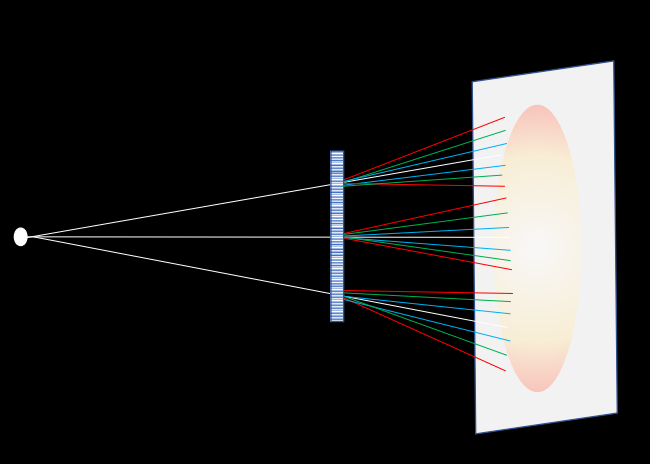
\includegraphics[width=0.4\linewidth]{IM reticolo non collimato}
  \caption{Situazione in cui il fascio di luce non risulta collimato}
\end{figure}


Una volta ottenuti dei fasci collimati possiamo utilizzare la relazione:

\begin{equation}
d (\sin \theta + \sin \alpha_n(\lambda)) = n \lambda
\end{equation}

In cui $d$ è il passo del reticolo, $\theta$ è l'angolo di incidenza rispetto alla normale del reticolo, $\alpha_n(\lambda)$ è l'angolo a cui si trova la lunghezza d'onda analizzata, $n$ è l'ordine che si sta analizzando e $\lambda$ è la lunghezza d'onda.

\vspace{3mm}

Se ci poniamo in condizioni di ortogonalità tra la luce e il reticolo il valore di $\sin \theta$ diventa 0 e possiamo quindi semplificare ottenendo:

\begin{equation}
d \sin \alpha = n \lambda
\end{equation}

Un'altra condizione necessaria per poter visualizzare la diffrazione è il porsi in campo lontano, come visibile nelle Figure 2 e 3. Se ci si pone troppo vicini allo schermo le varie lunghezze d'onda non hanno il tempo di separarsi e si osserva quindi solo luce bianca. 

\vspace{3mm}

Definiamo campo lontano una condizione in cui $L << l$ dove $L$ è la distanza del reticolo dallo schermo (campo lontano) e $l$ è la porzione illuminata sul reticolo.


%immagine reticolo collimato corto
\begin{figure}[h!]
  \centering
  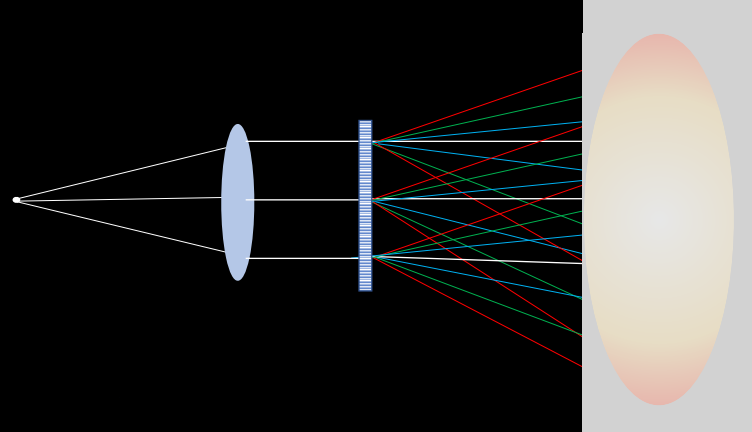
\includegraphics[width=0.4\linewidth]{IM reticolo collimato vicino}
  \caption{Situazione in cui lo schermo risulta troppo vicino}
\end{figure}

%immagine reticolo collimato lungo
\begin{figure}[h!]
  \centering
  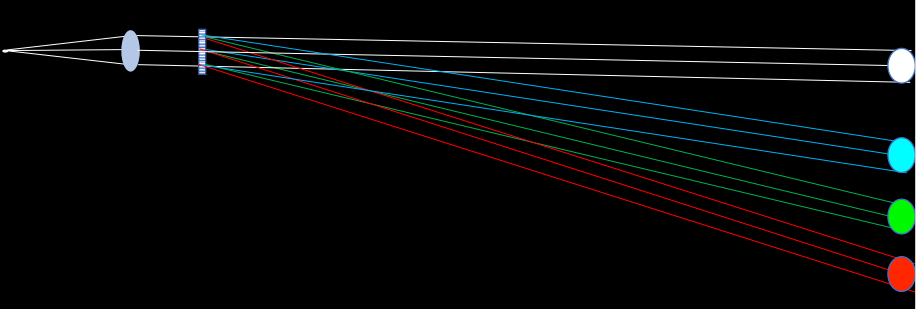
\includegraphics[width=0.4\linewidth]{IM reticolo collimato lontano}
  \caption{Situazione di campo lontano}
\end{figure}


\pagebreak
\section{Progettazione dell'esperienza}
Per questa esperienza ho utilizzato due reticoli, il primo di passo noto pari a $500 \; [righe/mm]$ mentre il secondo di passo ignoto. 

\vspace{3mm}

Come sorgenti luminose ho usato un puntatore laser di lunghezza d'onda ignota e una torcia. La torcia utilizzata ha, attaccata in fronte alla lampada, una lente mobile che, se estesa alla massima distanza, rende i raggi emessi paralleli rendendo la torcia adatta per le misure descritte.

\vspace{3mm}

Lo schermo usato è un muro che essendo, essendo non bianco, potrebbe aver leggermente falsato la visione del colore ma non ritengo ciò abbia influito in maniera significativa e non ne ho quindi  tenuto conto nell'analisi dati.

\vspace{3mm}

Per la presa delle misure della lunghezza ho usato un metro a nastro dalla portata di $3 \; m$ e dalla sensibilità del millimetro.

\section{Incertezza delle misure per la torcia}
Dato che l'immagine della torcia non risulta perfettamente netta ma ha delle leggere "sfocature" sui bordi esterni, ho deciso di prendere 5 misure della larghezza dell'immagine della torcia a una distanza di $2,25 \; m$ per ottenere, utilizzando la deviazione standard, una stima dell'incertezza sulle misure della torcia che è stata sommata in quadratura all'incertezza strumentale ottenendo il valore
\[ \sigma_D = 0,004 \; [m]\]
che è stato usato come incertezza sulle misure per le misure della torcia.

\clearpage

Riporto in Figura 4 la tabella contenente i dati.

%tabella incertezza torcia
\begin{figure}[h!]
  \centering
  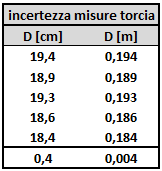
\includegraphics[width=0.25\linewidth]{IM tabella incertezza torcia}
  \caption{Dati usati per calcolare l'incertezza delle misure della torcia}
\end{figure}


\section{Misura della $\lambda_{laser}$}
Per calcolare la lunghezza d'onda del laser ho attaccatto il reticolo al bordo di un mobile posizionato parallelamente al muro. Ho quindi posizionato il laser attaccato al reticolo cercando di ottenere il più possibile una situazione di ortogonalità con quest'ultimo. Ho quindi proceduto ad accendere il laser e misurare la distanza tra il reticolo e il massimo (puntiforme) di ordine zero. Dopo avere annotato la distanza, chiamata $L$ in Figura 5, ho proceduto a misurare la distanza dell'ordine zero dai massimi (puntiformi) del primo e del secondo ordine (misure $D$ in Figura 5). 

\vspace{3mm}

Per l'analisi dati ho calcolato il valore di $\sin \alpha$  utilizzando la formula di carattere geometrico:

\begin{equation}
 \sin \alpha =\frac{L^2}{\sqrt{D^2 + L^2}}
\end{equation}

In cui ho propagato le incertezze ottenendo:

\begin{equation}
\sigma_{\sin \alpha} = \sqrt{\bigg( \frac{L^2 \sigma_D}{(D^2 + L^2)^{\frac{3}{2}}} \bigg)^2 + \bigg( \frac{L  D  \sigma_L}{(D^2 + L^2)^{\frac{3}{2}}} \bigg)^2} 
\end{equation}

Ho poi calcolato i valori delle singole $\lambda$ usando l'Equazione (5) derivata dall'Equazione (2) e, per ciascuna di esse, ho propagato l'errore tramite l'Equazione (6).

\begin{equation}
\lambda = \frac{D \sin \alpha}{n}
\end{equation}

\begin{equation}
\sigma_\lambda = \sqrt{\bigg( \frac{D \sigma_{\sin \alpha}}{n} \bigg)^2}
\end{equation}

Ho usato i risultati ottenuti per calcolare, usando una media pesata, il valore:
\[ \lambda_{laser} = 637.3 \pm 0.1 \; [nm] \]
Ritenendo che l'incertezza fosse troppo bassa ho deciso di calcolare la deviazione standard dei valori $\lambda$ e, tramite la somma in quadratura, unirla all'incertezza derivata dalla propagazione degli errori. 

\vspace{3mm}

Così facendo ho ottenuto un'incertezza che tenesse conto anche di possibili errori non strumentali, ad esempio il laser non perfettamente ortogonale o eventuali imprecisioni nelle misure data la conformazione della stanza. 

\vspace{3mm}

Il valore finale è risultato quindi essere:
\[ \lambda{laser} = 637 \pm 35 \; [nm] \]
Riporto in Figure 5 e 6 le tabelle con i dati grezzi, i risultati parziali e i valori finali.

%tabella laser 1
\begin{figure}[h!]
  \centering
  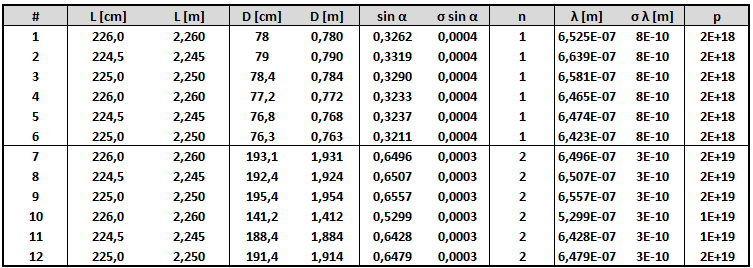
\includegraphics[width=1\linewidth]{IM tabella laser 1}
  \caption{Tabella contenente i dati del laser per il reticolo 1 e i risultati parziali}
\end{figure}

%risultati laser 1
\begin{figure}[h!]
  \centering
  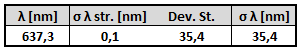
\includegraphics[width=0.4\linewidth]{IM risultati laser 1}
  \caption{Risultati misura $\lambda_{laser}$}
\end{figure}




\pagebreak
\section{Misura del passo del secondo reticolo}
Per la misura del passo del secondo reticolo ho scambiato il reticolo utilizzato e ho proceduto in maniera analoga a quanto fatto nella misura precedente. Per l'analisi dati ho proceduto analogamente fino al calcolo di $\sin \alpha$. Ho quindi usato l'Equazione (7), sempre derivata dall'Equazione (2), per il calcolo di $d$ e ho propagato gli errori come mostrato in Equazione (8).

\begin{equation}
 d = \frac{\lambda}{\sin \alpha}
\end{equation}

\begin{equation}
 \sigma_d = \sqrt{ \bigg( \frac{\sigma_\lambda}{\sin \alpha} \bigg)^2 + \bigg( \frac{- \lambda \sigma_{\sin \alpha}}{\sin^2 \alpha} \bigg)^2 }
\end{equation}

Nelle equazioni appena scitte non è presente $n$, dato che il secondo ordine non era visibile e tutte le misure risultano prese al primo ordine.

\vspace{3mm}

Ho quindi usato una media pesata e la deviazione standard come già precedentemente fatto per $\lambda$ ottenendo il valore:
\[ d = 994 \pm 87 \; [nm] \]
da cui otteniamo:
\[ d = 1006 \pm 89 \; [righe/mm] \]
Riporto in Figure 7 e 8 le tabelle con i dati grezzi, i risultati parziali e i valori finali.

%tabella laser 2
\begin{figure}[h!]
  \centering
  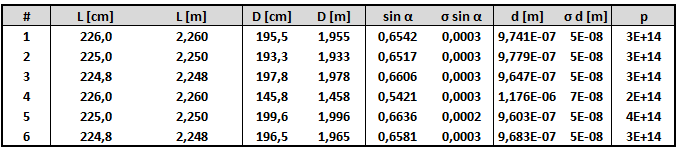
\includegraphics[width=1\linewidth]{IM tabella laser 2}
  \caption{Tabella contenente i dati del laser per il reticolo 2 e i risultati parziali}
\end{figure}

%risultati laser 2
\begin{figure}[h!]
  \centering
  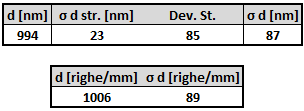
\includegraphics[width=0.4\linewidth]{IM risultati laser 2}
  \caption{Risultati misura passo del reticolo}
\end{figure}




\pagebreak
\section{Misure dello spettro della torcia}
\subsection{Primo reticolo}
Al contrario delle misure del laser, per le misure dello spettro della torcia mi sono spostato in una stanza buia per riuscire a vedere meglio la luce. Ho posizionato la torcia su una scatola e ho attaccato la torcia alla scatola utilizzando dello scotch. Ho successivamente posizionato il reticolo in prossimità della torcia e l'ho fissato saldamente con altro scotch.

\vspace{3mm}

Per questa misura ho raccolto la distanza tra il reticolo e il centro dell'immagine della torcia. Per maggiore precisione nelle misure della posizione delle bande colorate ho misurato la distanza tra il bordo sinistro dell'immagine di ordine 0 e il bordo sinistro delle immagini ai vari ordini per gli spettri a destra e viceversa per gli spettri a sinistra. 

\vspace{3mm}
Ho deciso di prendere misure per i colori rosso, arancione, giallo e blu dato che, ruotando il reticolo, i quadrati della torcia non si sovrapponevano perfettamente e dagli angoli mi pareva di vedere i colori precedenti con l'aggiunta del verde (vedere Figura 10).%numero figura
 
\vspace{3mm}

Purtroppo il verde non risultava ben visibile al primo ordine e non sono riuscito quindi ad inserirlo nella presa dati mentre riguardo al giallo non sono risucito a distinguerlo correttamente il giallo e ho segnato quindi solo.

%torcia dritta
\begin{figure}[h!]
  \centering
  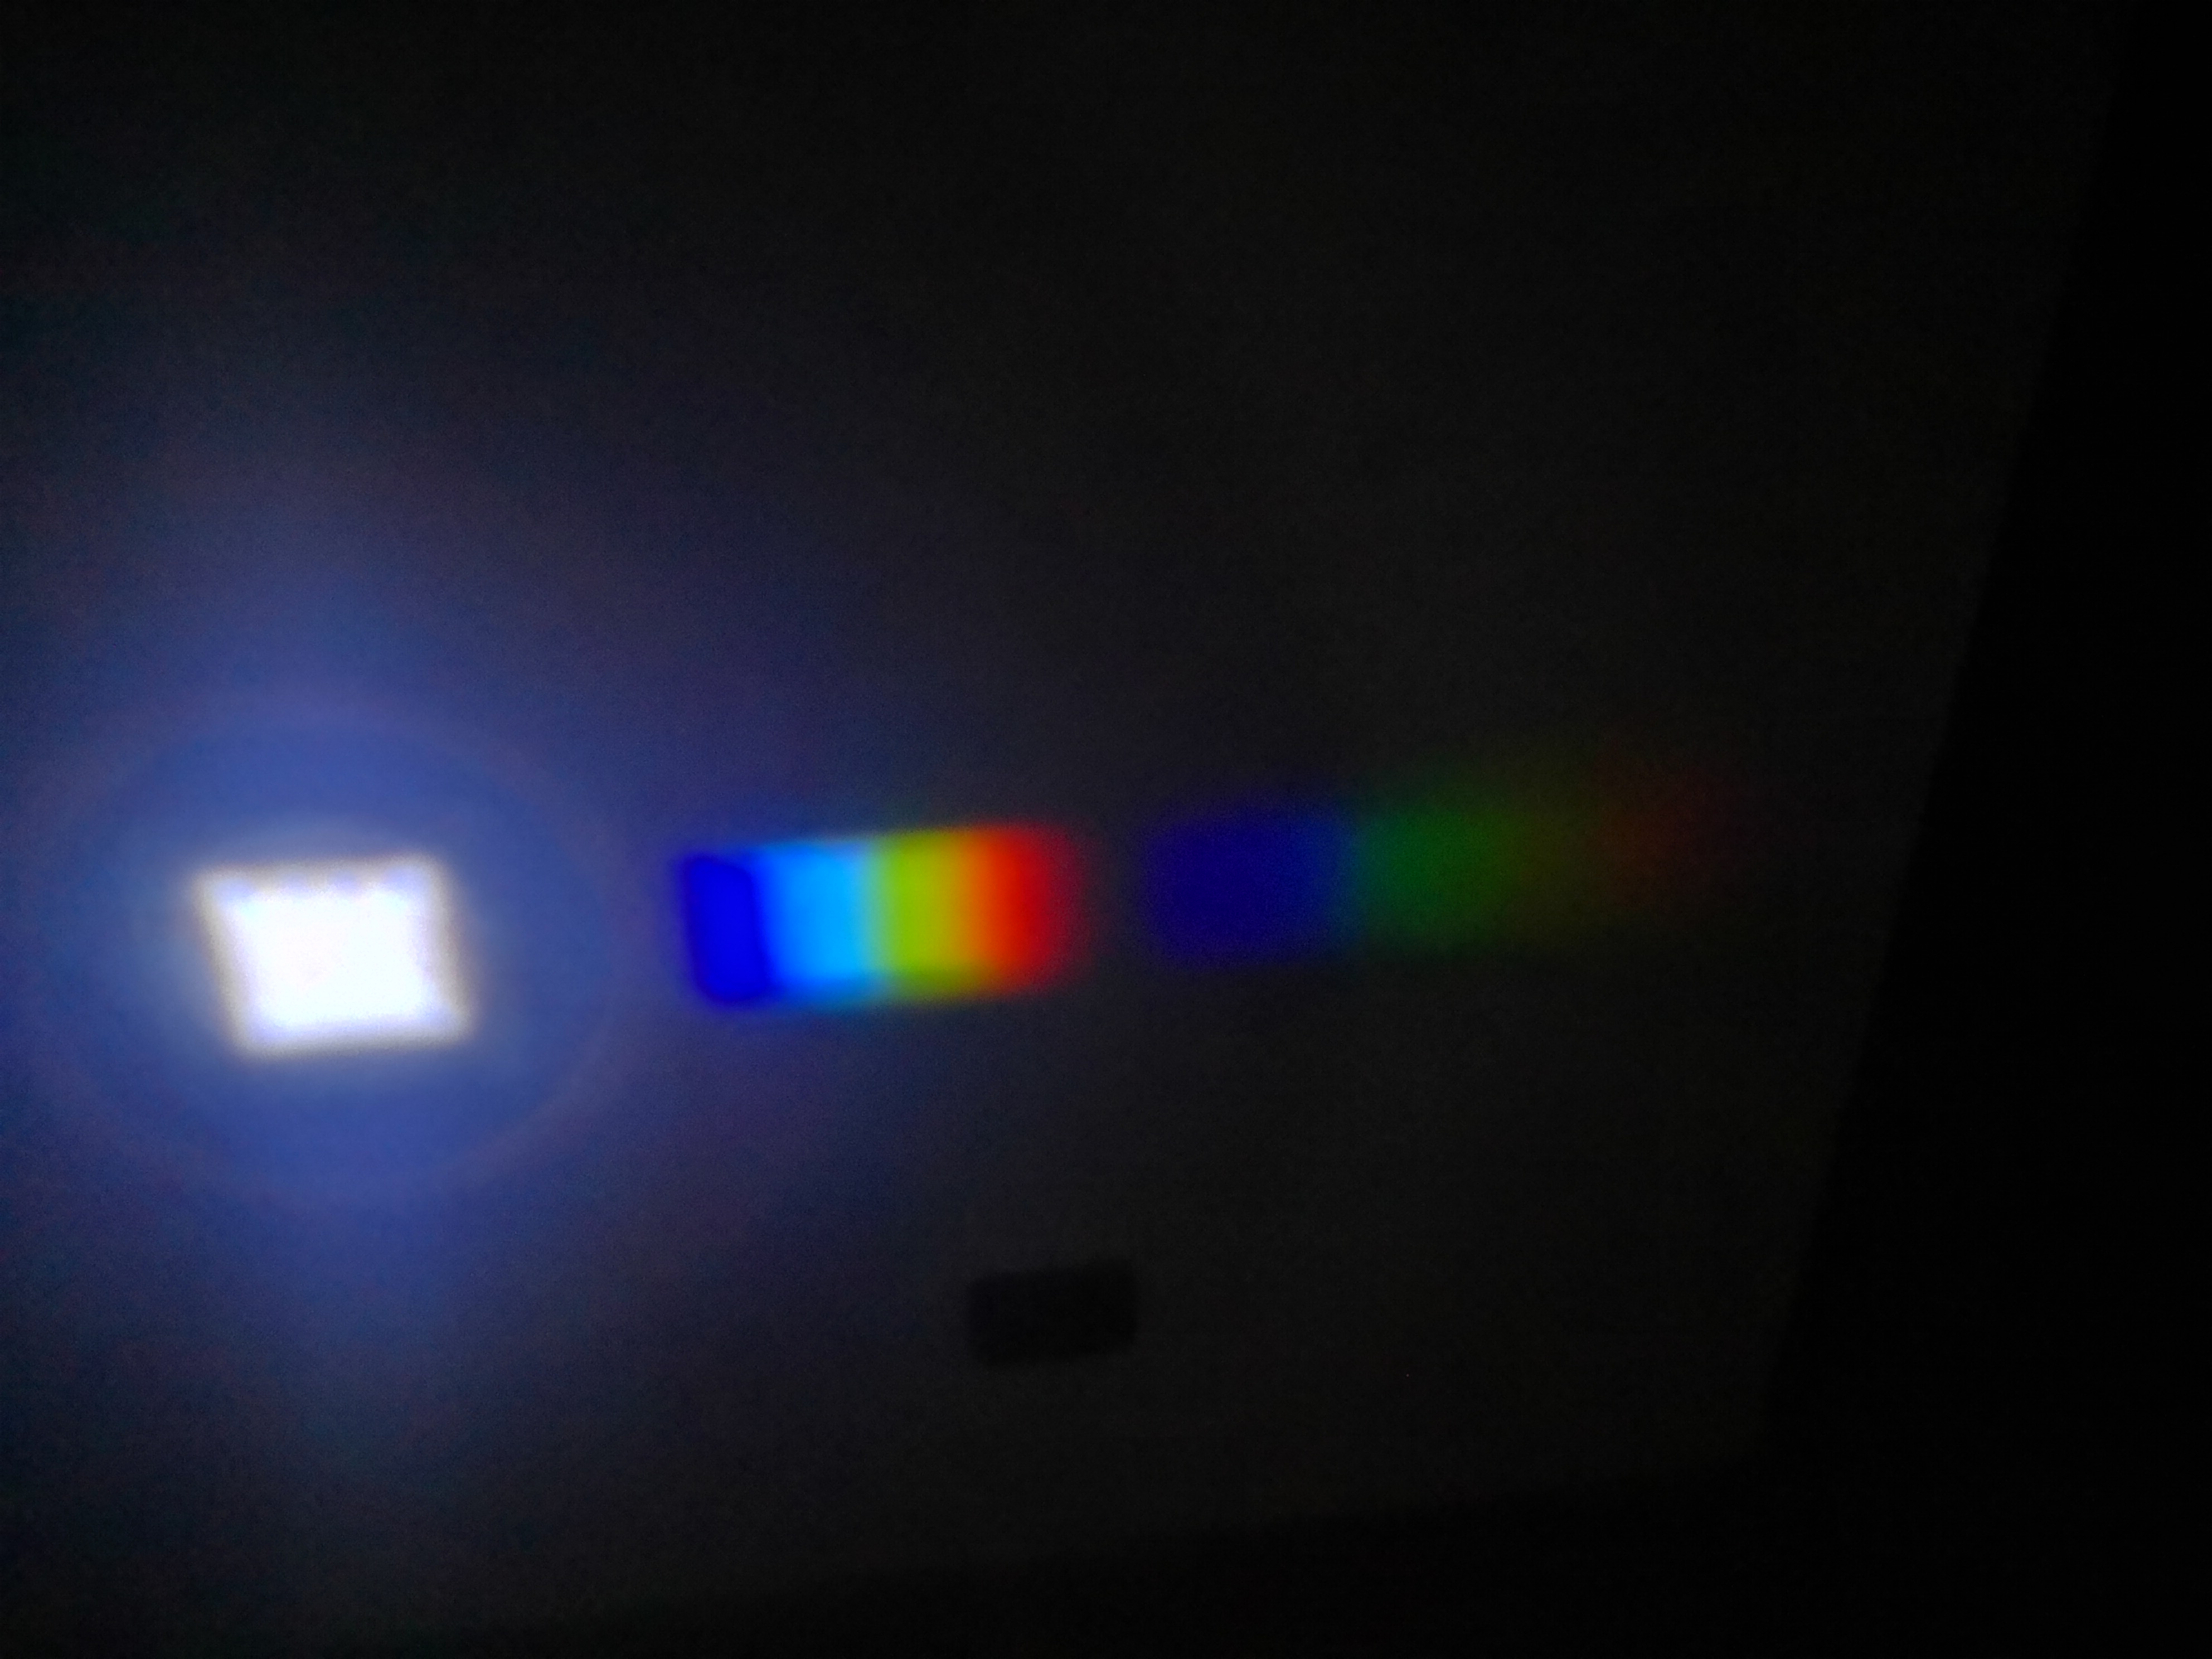
\includegraphics[width=0.4\linewidth]{IM torcia}
  \caption{Immagine primo e secondo ordine destro dello spettro della torcia}
\end{figure}

%torcia storta
\begin{figure}[h!]
  \centering
  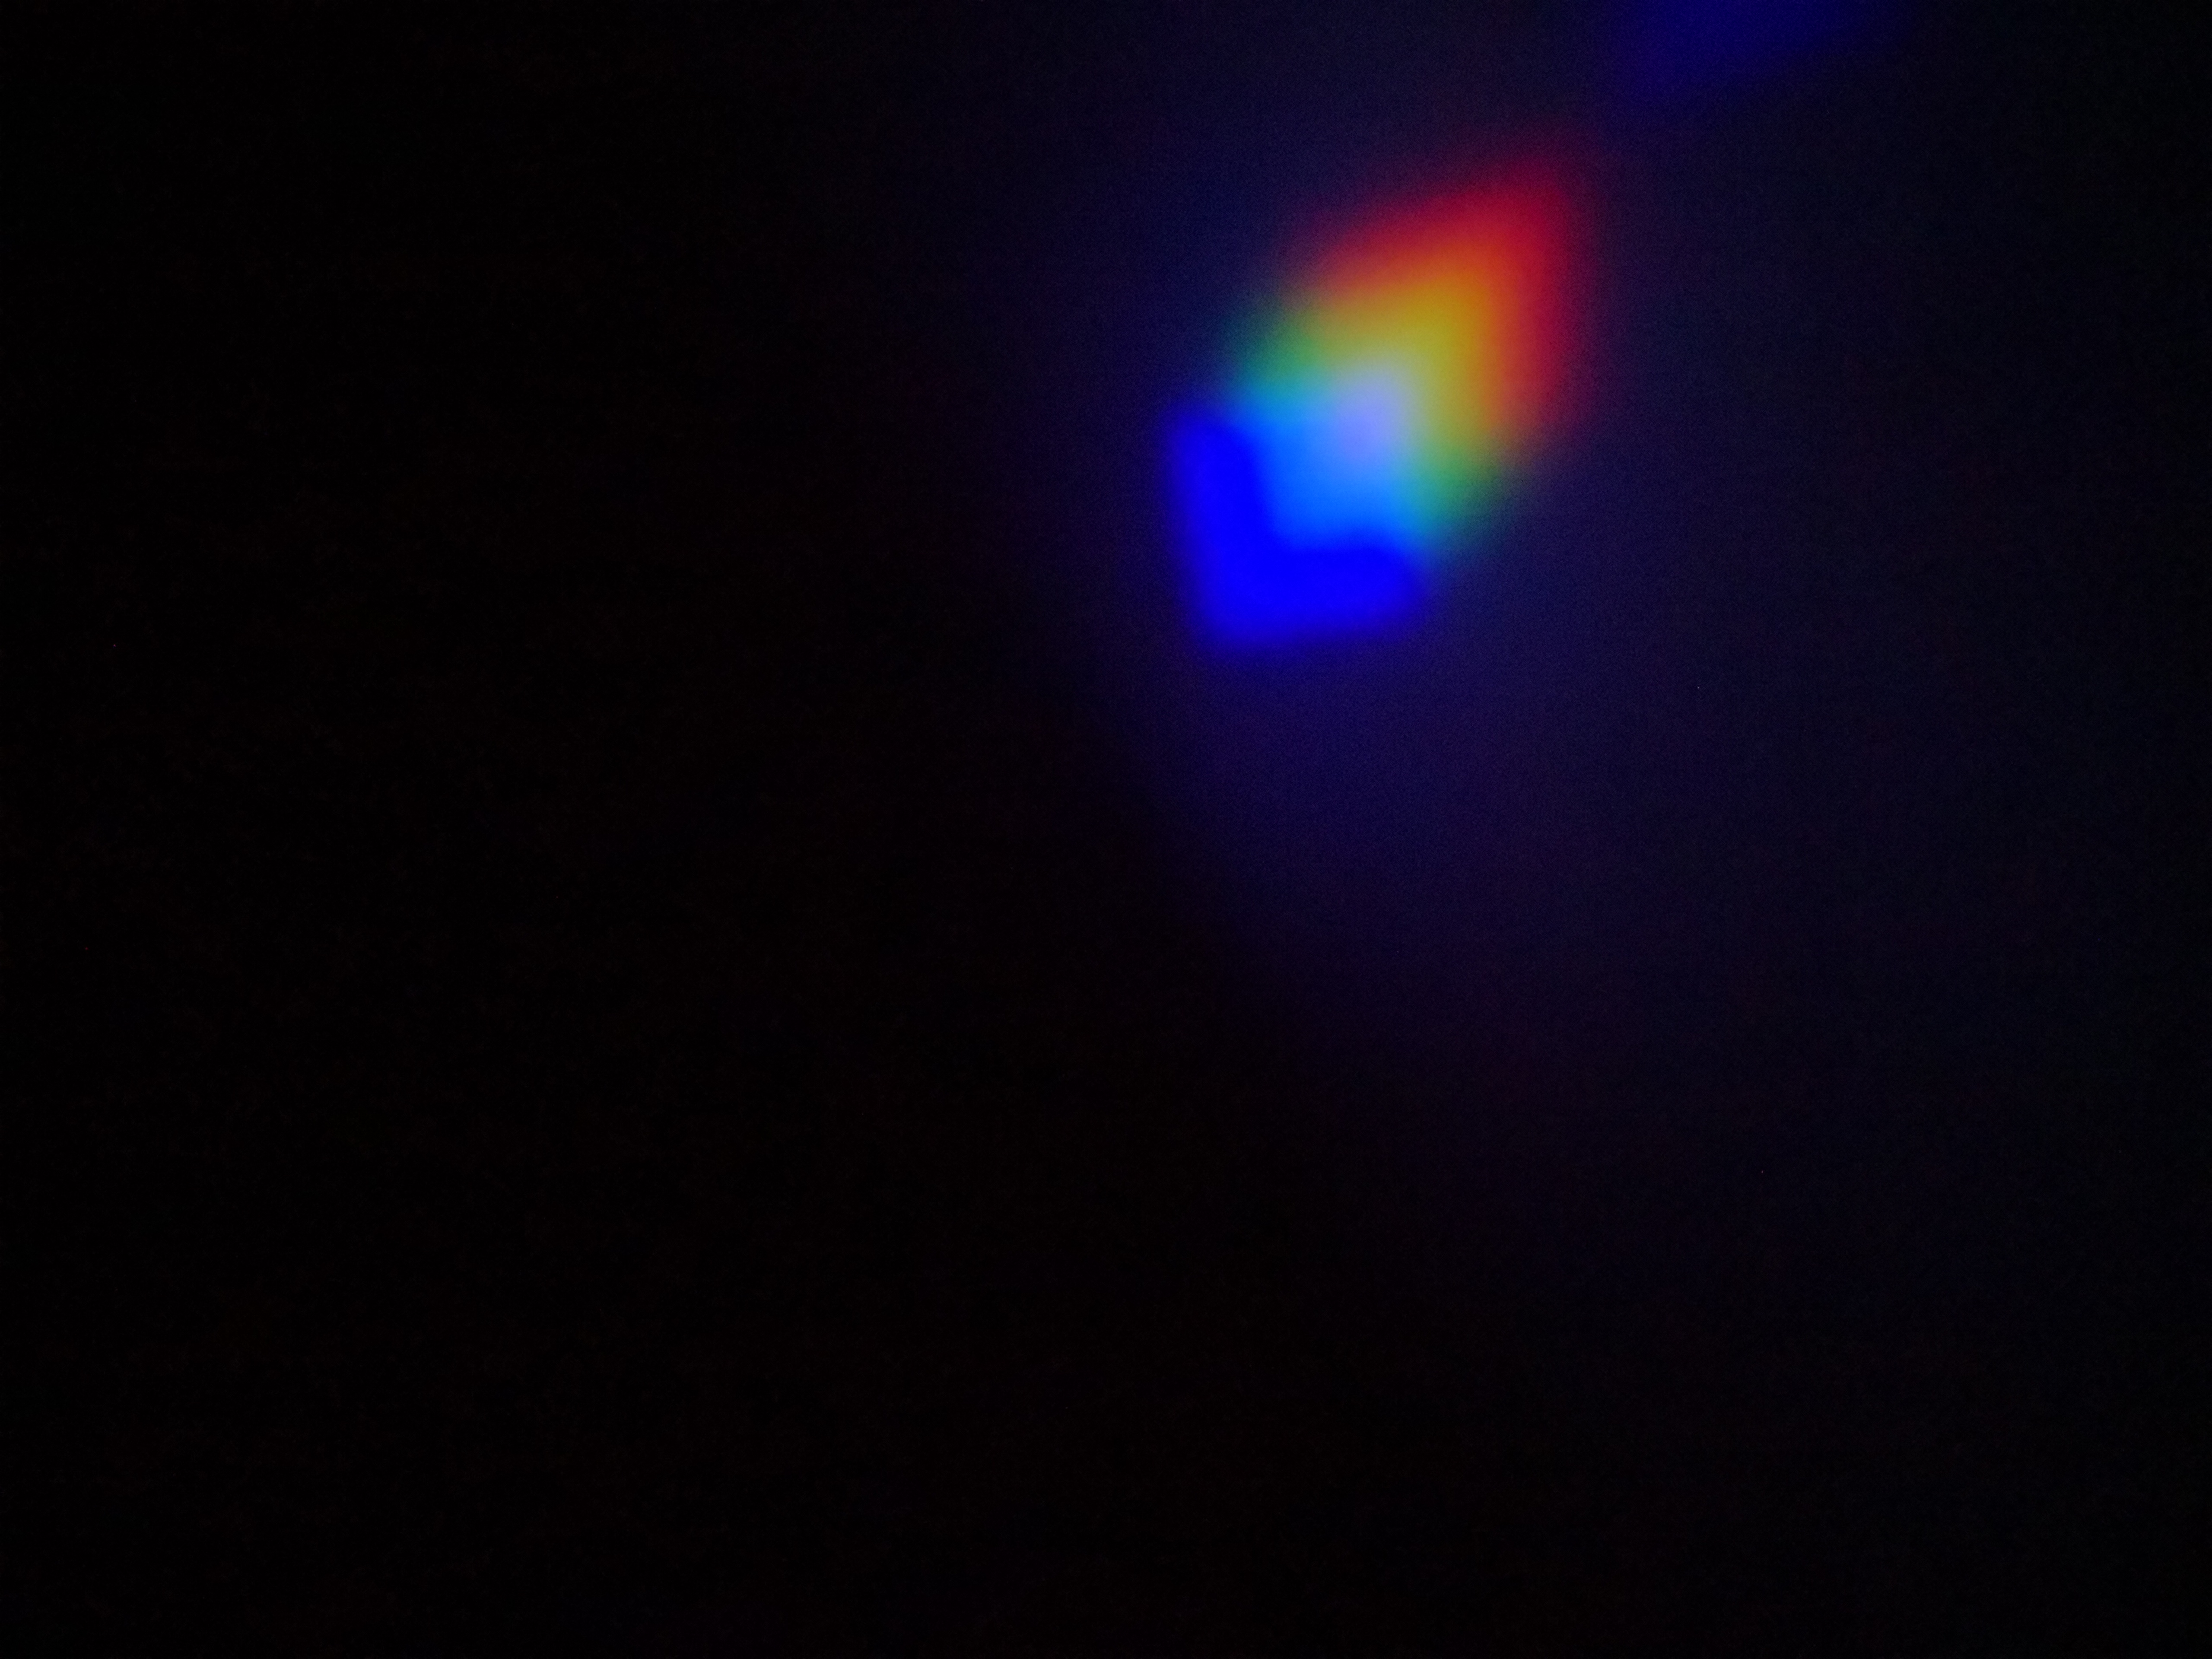
\includegraphics[width=0.4\linewidth]{IM torcia storta}
  \caption{Spettro ruotando il reticolo, in realtà si distingue chiaramente un quadrato blu e una serie di quadrati sfumati tra il verde e il rosso che sembrano essere verde giallo arancio e rosso.}
\end{figure}

Per l'analisi dei dati ho proceduto analogamente a quanto fatto per la determinazione di $\lambda_{laser}$, ma l'incertezza strumentale usata è quella descritta in Incertezza delle misure per la torcia.
I valori ottenuti sono:

\vspace{3mm}

\begin{centering}
$blu:$ \;\;\;\;\;\; $\lambda_1 = 445 \pm 10\; [nm]$

$giallo:$ \;\; $\lambda_1 = 623 \pm 10\; [nm]$ 

$arancio:$ $\lambda_1 = 606 \pm 67\; [nm]$ 

 $rosso:$ \;\;\; $\lambda_1 = 652 \pm 63\; [nm]$ 

\end{centering}

\vspace{3mm}

Riporto nelle Figure da 11 a 18 le tabelle con i datil,i risultati parziali e i valori finali.

%tabella blu 1
\begin{figure}[h!]
  \centering
  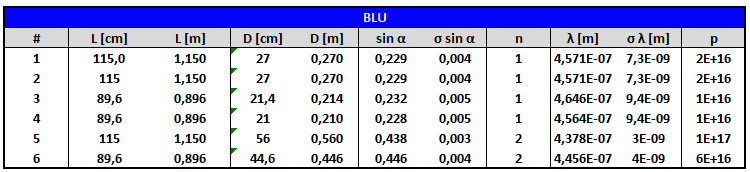
\includegraphics[width=1\linewidth]{IM tabella blu 1}
  \caption{Tabella blu 1}
\end{figure}

%risultati blu 1
\begin{figure}[h!]
  \centering
  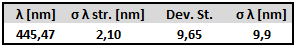
\includegraphics[width=0.4\linewidth]{IM risultati blu 1}
  \caption{Risultati blu 1}
\end{figure}

%tabella giallo 1
\begin{figure}[h!]
  \centering
  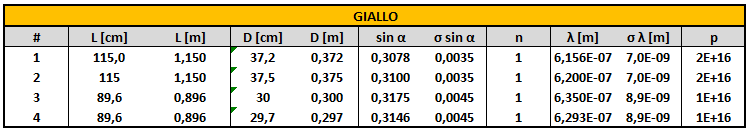
\includegraphics[width=1\linewidth]{IM tabella giallo 1}
  \caption{Tabella giallo 1}
\end{figure}

%risultati giallo 1
\begin{figure}[h!]
  \centering
  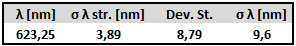
\includegraphics[width=0.4\linewidth]{IM risultati giallo 1}
  \caption{Risultati giallo 1}
\end{figure}

%tabella arancio 1
\begin{figure}[h!]
  \centering
  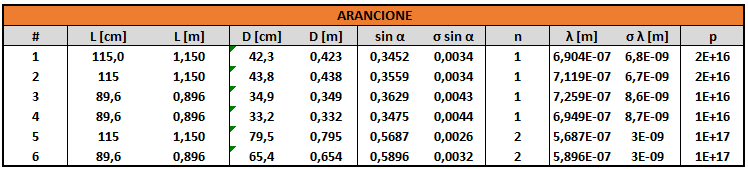
\includegraphics[width=1\linewidth]{IM tabella arancio 1}
  \caption{Tabella arancione 1}
\end{figure}

%risultati arancio 1
\begin{figure}[h!]
  \centering
  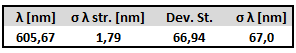
\includegraphics[width=0.4\linewidth]{IM risultati arancio 1}
  \caption{Risultati arancione 1}
\end{figure}

%tabella rosso 1
\begin{figure}[h!]
  \centering
  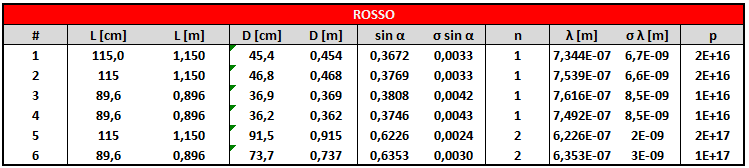
\includegraphics[width=1\linewidth]{IM tabella rosso 1}
  \caption{Tabella rosso 1}
\end{figure}

%risultati rosso 1
\begin{figure}[h!]
  \centering
  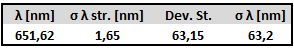
\includegraphics[width=0.4\linewidth]{IM risultati rosso 1}
  \caption{Risultati rosso 1}
\end{figure}


\pagebreak%help
\subsection{Secondo reticolo}
Per l'analisi effettuata con il secondo reticolo mi sono limitato a cambiare il reticolo davanti alla torcia. 

Nell'analisi dei dati ho tuttavia tenuto conto dell'ncertezza sul passo del reticolo e ho quindi propagato l'errore tramite la formula:

\begin{equation}
 \lambda = \sqrt{ \bigg( \frac{\sigma_d \sin \alpha}{n} \bigg)^2 + \bigg( \frac{d \sigma_{\sin \alpha}}{n} \bigg)^2 }
\end{equation}

I valori ottenuti sono:

\vspace{3mm}

\begin{centering}
$blu:$ \;\;\;\;\;\; $\lambda_1 = 448 \pm 21\; [nm]$

$giallo:$ \;\; $\lambda_1 = 586 \pm 29\; [nm]$ 

$arancio:$ $\lambda_1 = 613 \pm 30\; [nm]$ 

 $rosso:$ \;\;\; $\lambda_1 = 646 \pm 32\; [nm]$ 

\end{centering}

\vspace{3mm}

Riporto nelle Figure da 19 a 26 le tabelle con i datil,i risultati parziali e i valori finali.

%tabella blu 2
\begin{figure}[h!]
  \centering
  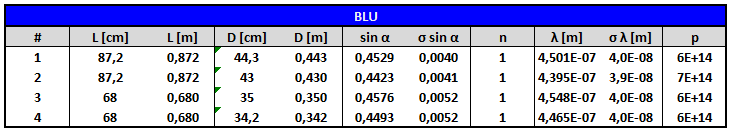
\includegraphics[width=1\linewidth]{IM tabella blu 2}
  \caption{Tabella blu 2}
\end{figure}

%risultati blu 2
\begin{figure}[h!]
  \centering
  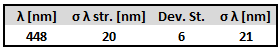
\includegraphics[width=0.4\linewidth]{IM risultati blu 2}
  \caption{Risultati blu 2}
\end{figure}

%tabella giallo 2
\begin{figure}[h!]
  \centering
  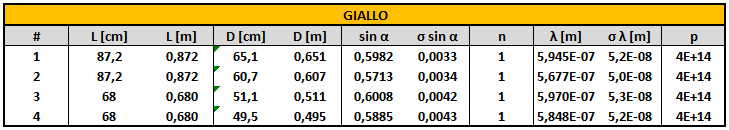
\includegraphics[width=1\linewidth]{IM tabella giallo 2}
  \caption{Tabella giallo 2}
\end{figure}

%risultati giallo 2
\begin{figure}[h!]
  \centering
  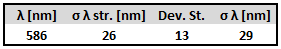
\includegraphics[width=0.4\linewidth]{IM risultati giallo 2}
  \caption{Risultati giallo 2}
\end{figure}

%tabella arancio 2
\begin{figure}[h!]
  \centering
  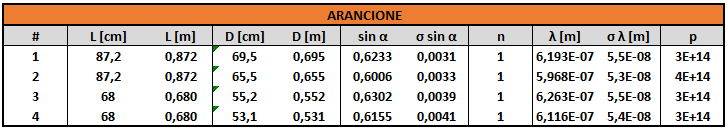
\includegraphics[width=1\linewidth]{IM tabella arancio 2}
  \caption{Tabella arancione 2}
\end{figure}

%risultati arancio 2
\begin{figure}[h!]
  \centering
  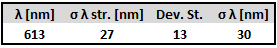
\includegraphics[width=0.4\linewidth]{IM risultati arancio 2}
  \caption{Risultati arancione 2}
\end{figure}

%tabella rosso 2
\begin{figure}[h!]
  \centering
  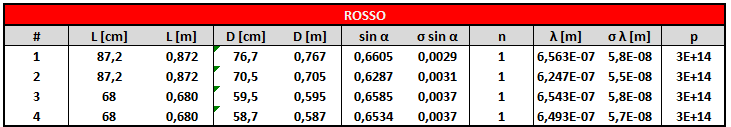
\includegraphics[width=1\linewidth]{IM tabella rosso 2}
  \caption{Tabella rosso 2}
\end{figure}

\clearpage
%risultati rosso 2
\begin{figure}[t]
  \centering
  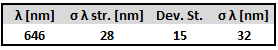
\includegraphics[width=0.4\linewidth]{IM risultati rosso 2}
  \caption{Risultati rosso 2}
\end{figure}


\subsection{Analisi dei risultati}
Riporto nelle Figure 27 e 28 la comparazione dei risultati in tabella e in grafico. Come è possibile notare tutte le misure sono compatibili tra loro con l'eccezione del giallo del reticolo 1. Ho fatto una comparazione dei colori utilizzando il sito \textit{wolframalpha.com} per convertire le lunghezze d'onda ottenute nei rispettivi colori. Ho notato che le misure del blu tendono leggermente al violetto al contrario di quanto visibile con la torcia. La misura del giallo del reticolo 1 risulta essere tra un arancione scuroe un rosso vivace e ritengo sia quindi errata. Per finire, sia le misure dell'arancione e del  rosso risultano leggermente più scure, ipotizzo ciò sia dovuto alla maggiore difficolta, riscontrata durante la presa dati, nel trovare un confine netto nel passaggio giallo-arancio e arancio-rosso.


%comparazione risultati
\begin{figure}[h!]
  \centering
  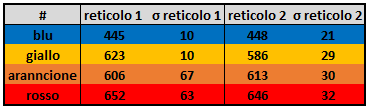
\includegraphics[width=0.5\linewidth]{IM comparazione risultati}
  \caption{Tabella di comparazione dei risultati}
\end{figure}

%grafico risultati
\begin{figure}[h!] 
  \centering
  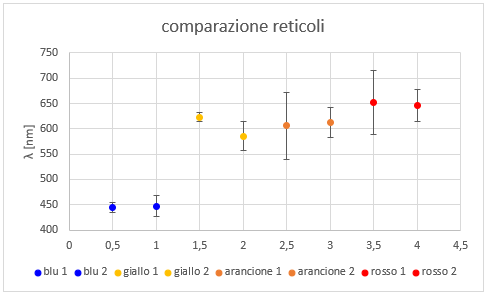
\includegraphics[width=0.6\linewidth]{IM grafico risultati}
  \caption{Grafico di comparazione dei risultati}
\end{figure}



\pagebreak
\section{Conclusioni}
Le misure eseguite con il laser hanno prodotto risultati soddisfacenti e plausibili con il valore vero delle lunghezze d'onda dei colori osservati. Anche usando \textit{wolframalpha.com} il colore della lunghezza d'onda calcolato sembra simile a quello della luce emessa dal laser. Per quanto riguarda il passo del secondo reticolo il numero di fenditure per $mm$ circa doppio rispetto al primo spiegerebbe la posizione del primo ordine del secondo reticolo in posizione simile a quella del secondo ordine del primo reticolo. 

\vspace{3mm}

Ritengo plausibili i risultati dello spettro della torcia con l'eccezione della lunghezza d'onda del giallo per il primo reticolo che, come già specificato nella Sezione 6.3, risulterebbe essere di colorazione rossa.
\end{document}